\documentclass{report}
\usepackage[utf8x]{inputenc}
%\usepackage[mac]{inputenc}

\usepackage{url} \urlstyle{sf}
\usepackage[a4paper,margin=1.9cm]{geometry}
\usepackage{xspace}
\usepackage[francais,american]{babel}
\usepackage{palatino}
\usepackage{bibtopic}
\usepackage{graphicx}
\usepackage{enumitem}
\usepackage{dot2texi}

\newcommand{\kaapi}{\textsc{X}-Kaapi\xspace}
%%\newcommand{\new}{\hspace*{10ex}\textbf{\textsc{New in \kaapi.}~\\}\xspace}
\newcommand{\new}{}
\newcommand{\inote}[1]{\textit{\textbf{  \center \hrule Implementation note\hrule}}\vspace*{1ex}\textit{#1}\vspace{1ex} \hrule\vspace*{2ex}}

%\newcounter{subsubsection}[subsection]
\renewcommand{\subsubsection}[1]{~\\ \addtocounter{subsubsection}{1} \noindent\textit{
%\textbf{\thesubsection.
\thesubsubsection. #1\\}}


\newcounter{subsubsubsection}[subsubsection]
\newcommand{\subsubsubsection}[1]{~\\ \addtocounter{subsubsubsection}{1} \noindent\textit{\textbf{\thesubsubsection.\thesubsubsubsection. #1\\}}}
\newtheorem{proposition}{Proposition}

%\renewcommand{\subsubsection}[1]{~\\ \addtocounter{subsubsection}{1} \noindent\textit{\textbf{\thesubsubsection\hspec #1\\}}}

\begin{document}

\title{Specification X-Kaapi}
\author{V. Danjean, T. Gautier, C. Laferrière}
\date{\today}
\maketitle

%%%
%%%
%%%
\newpage
\chapter{Introduction}


\section{Histoire}
Un peu d'histoire pour expliquer où nous en sommes.
En 1999, le 22 septembre, avec la thèse de François Galilée, la spécification d'Athapascan était posée: Fork + Shared + les modes et droits d'accès r, w, rw, cw ainsi que les modes postponed (rp,wp, rpwp, cwp). Une implémentation C++ complète a existé (sisi). Le coût a l'exécution était énorme : environ 10000 appels de fonction C pour 1 fork sans paramètre. Ceux-ci s'expliquaient de deux manières: 1/ un algorithme de terminaison distribuée était utilisé pour calcul la fin d'accès à une version pour déclencher les calculs sur la version suivante ; 2/ les choix des structures de données ainsi que leur allocation dans le tas ; 3/ le mauvais couplage entre la couche de communication thread safe Athapscan-0 et l'implémentation d'Athapascan-1 au dessus. Bien qu'en théorie, les algorithmes de cette implémentation distribuée devaient permettre d'avoir du bon speedup, en pratique il fallait avoir des calculs à très gros grain. L'ordonnancement était basé sur des variations autour du vol de travail avec des heuristiques pour permettre de contrôler l'utilisation mémoire, ou bien par ordonnancement de type statique d'un graphe de flot de données mais aucune perf n'a pu être observée.

Quelques semaines plus tard, le 14 décembre 1999, Mathias Doreille montrait dans sa thèse qu'il était possible d'avoir de très bon speedup sur des programmes ordonnancés par une variation d'un algorithme de type ETF et en utilisant une implémentation adhoc très légère directement au dessus de MPI mais incomplète vis-à-vis des spécifications d'Athapascan-1. L'ordonnancement local des messages et du calcul ne permettait pas d'avoir des performances raisonnables sur des programmes du type itératifs (jacobi, poisson) normaux (sans augmentation complexe / artificielle du grain).

En 2004, Rémi Revire a montré la faisabilité d'avoir une implémentation plus efficace permettant à la fois un ordonnancement par vol de travail et par ordonnancement de graphe en se basant sur une implémentation qui, grâce à l'ordre d'exécution quasi séquentiel d'un programme Athapascan, permet de gérer le cycle de vie des tâches et objets partagés en rapport à leurs portées de déclaration : la gestion par pile de l'exécution des programmes séquentiels était retrouvée ! Néanmoins, l'algorithme de terminaison du calcul distribué (non plus de la fin d'utilisation d'une version) était encore mal conçu, mais heureusement n'intervenait que pour déterminer la terminaison globale de l'exécution des processus.
Du point de vu des performances, l'implémentation se basait sur l'utilisation de lock pour verrouiller l'accès à certaines données lors des opérations de vols. Le partitionnement statique du graphe utilisait Scotch et était à l'état de prototype instable. L'ensemble était basé sur une couche de communication appelée Inuktitut qui permettait de communiquer par envoi/réception de messages actifs. 
Laurent Pigeon avait implanté un ensemble d'algorithmes pour la diffusion parallèle de message durant son master.
Lors d'un stage d'été, Xavier Besseron avait implanté le côté communication sur architecture hétérogène en utilisant soit un protocol de type Xdr (eXternal data representation), soit de type ASN.
Lors de son stage, Everton Hermann a effectué le portage d'Inuktitut sur Myrinet.
Le coût de cette implantation était d'environ 1000 appels de fonction C pour 1 fork (toujours sans paramètre).

En 2005, Kaapi est née des cendres d'Athapascan \& Inuktitut : une évaluation synthétique aurait été "ça marche pas trop mal, code de niveau prototype de recherche, mais peut mieux faire"
Plus précisément~:
\begin{itemize}
\item peu de support du côté d'Inuktitut qui avait été conçu pour servir à la conception de Taktuk (1ère version hélas très bogguée en C++) ou des outils ka-XXX pour la diffusion de fichiers.
\item 3 protocols de communication dans Inuktitut: active message, write \& signal (idem active message mais avec une allocation par la couche de comm des données reçues dans l'espace mémoire utilisateur) et une variante allocate \& write \& signal bien adaptée à un portage de la couche de comm directement au dessus de CORBA.
\item la portée des structures de données dans Athapscan n'était pas encore bien comprise, leur gestion nécessitait encore l'utilisation de locks.
\item l'algorithme de vol était décomposé en trois endroits : soit le vol effectif d'une tâche lors d'une requête local, soit lors vol suite à une requête à distance, soit le réveil d'un thread ce qui posait pas mal de problème de "stabilité" de celui-ci en cas de modification (...) En pratique toute tentative de modification d'une partie du vol de tâches ou du choix du reveil d'un thread était source de longues heures de débug...
\end{itemize}

Beaucoup de concepts avait été validés (couplage ordo statique / vol de travail) mais l'ensemble des sources étaient difficilement abordables par les étudiants arrivant sur le projet. En 2005, il fut donc fait les choix suivants~:
\begin{enumerate}
\item récupération d'Inuktitut et suppression du code non essentiel: protocol message actif
\item lors du stage d'Everton Hermann il a été vu qu'un fonctionnement de la couche de message par vol de travail permettait simplement d'agréger des messages vers le même destinataire, de plus elle était original dans le sens ou la fenêtre d'aggrégation dépendait de l'activité réseau...
\item une même opération pour le vol de tâche ou le réveil de thread: la fonction de vol prend en entrée un thread et retourne un thread ! Cela a l'avantage d'être simple et uniforme : dans le premier cas, un objet thread est volé et le thread résultat est rempli par la tâche volée, dans le second cas un objet processeur est volé et il retourne le thread à réveiller. 
\item la notion de graphe de flot de données (application) doit être découpé du vol de travail (ordonnancement), l'ordonnancement de Kaapi se base donc sur un ensemble de threads qui peuvent être volés, les threads pouvaient être directement du code applicatif ou bien structurés par pile de tâches. En pratique, seul la deuxième possibilité a été utilisé, même à travers les algorithmes adaptatifs de Daouda. Cette structuration a permis de réduire l'utilisation de verrou dans l'implémentation.
\item une conception uniforme des objets pouvant être sérialisés et qui sont représentés par leur "format" : les data ou les threads possèdent un format. La couche API Athapascan génère automatique avec un ensemble d'expression template les objets formats en fonction du type des objets à sérialiser.
\item la capacité d'interagir avec l'exécution par l'envoi de signaux : SIGSTOP, SIGSTOP, ou encore SIGKILL.
\item et enfin, un prototype pour la collection de statistique d'exécution des processus et l'enregistrement d'événement dans des fichiers de trace. 
\end{enumerate}

Les derniers points 5/ et 6/ ont facilité en partie l'implémentation des protocoles de tolérance aux pannes : arrêt des activités et sérialisation de facto des threads.

L'interface de programmation de la couche de communication n'a pas bougé depuis 2005, en revanche un développement a été nécessaire pour permettre de faire communiquer un ensemble de processus dynamiques et rendre robuste la panne d'un ou plusieurs processus sans provoquer l'arrêt les autres de manière non contrôlée. De plus, cette couche est "multi-réseau" avec une sélection du réseau à la source en fonction du destinataire qui a l'avantage d'être simple, mais n'est pas forcément très performante.

Cette version de Kaapi a permis de reporter successivement les 3 plugtest 2006 (non officiel dans le sens que nous n'avons pas été classé comme les autres car non java-compliant, mais les résultats étaient bien devant les autres), 2007 et 2008.
Pour 2009 : le ETSI Grid@Work plugtest s'oriente vers les aspects uniquement déploiement... on ne participera pas.

Mes critiques sont :
\begin{enumerate}
\item code gros devenant gros ne facilitant pas la gestion de l' "histoire" pour les nouveaux arrivants.
\item les perfs de l'aspect purement multi-core / SMP / many-core peuvent être meilleur
\item les choix des routes / des interfaces dans la couche communication doit être amélioré. N'ayant pas de travaux de recherche (thèse) sur ce point, nous n'arrivons pas à nous reposer sur une couche externe "portable" et robuste (grid, cluster, ...) ayant des capacités de dynamicité / robustesse en cas de panne qui soient suffisantes.
\item l'absence d'une interface permettant de gérer la transparence référentielle des objets partagés, i.e. être capable d'accéder en lecture ou écriture aux objets quel que soit le site d'exécution. Ce point est délicat et doit être guidé par certaines décisions d'ordonnancement.
\item l'absence de la notion de collection d'objets distribués (utilisant un support comme décrit dans le point 4/ ci-dessus) permettant la description de la plupart des  algorithmes en calcul scientique pour lesquels il serait intéressant d'avoir à manipuler des tableaux multi-dimmensionels d'objets "shared".
\item absence d'une couche "serveurs de stockage fiable" pour les protocoles de tolérance aux pannes... De même que pour 3, il est difficile de trouver du source dans ce domaine qui permettent de bonne performance. Néanmoins une évaluation des outils récents seraient à refaire (la dernière date de 2006-2007).
\item mauvais couplage des algorithmes adaptatifs.
\end{enumerate}

Début 2009: naissance de X-Kaapi pour répondre aux points 2/ et 6/ tout en facilitant le portage de X-Kaapi sur des systèmes embarqués dans le cadre de nos collaborations avec ST, i.e. en utilisant du C !



%%%
%%%
%%%
\newpage
\section{Objectifs et problématiques}
Les objectifs de X-Kaapi sont de capitaliser le savoir faire que nous avons eu en vu de cibler de nouvelles architectures (pour nous) et de nouvelles applications.
Le contexte technologique est induit par des architectures à mémoire hiérarchique composées par des processeurs de type multi-core ou many-core ou du domaine de l'embarqué (MpSoC). Ces processeurs communiquent par de la mémoire ou un réseau. La latence d'accès à la mémoire varie fortement en fonction de la distance entre la données et le cœur qui y accède. L'environnement d'exécution disponible n'est peut-être pas aussi complet que celui d'un PC actuel. En particulier en ce qui concerne l'ordonnancement de threads, la gestion mémoire (pas de mémoire virtuelle, taille limité). Le nombre total de cœur peut être très important.

Les deux architectures cibles initiales sont :
\begin{itemize}
\item une bluegene : un nœud est composé d'un ensemble de cœurs partageant une mémoire local, partageant ou non une hiérarchie de caches. Le réseau d'interconnexion est de type grille 3D torique (sous contrainte de routage au bord en fonction d'une réservation partielle). Ce réseau n'est utilisé que pour les communication bi-point. La machine dispose aussi d'un réseau de diffusion (broadcast) et d'un réseau de synchronisation. La taille mémoire par nœud est limité (256MBytes ou 512MBytes). Les possibilités de l'OS sont à découvrir. La couche de communication DCMF disponible est de bas niveau et offre une communication de type messages actifs et lecture/écriture à distance. Les questions qui se posent sont liés à la capacité à traiter des handlers de communication en concurrence avec du calcul, la capacité du système à faire progresser les communications et à ordonnancement plusieurs threads.
\item MpSoC : la board ST composé de 4 cœurs ST 231 qui communiquent par des envois de message ou du partage d'objet (dans un sens très particulier) vers, et uniquement vers, le cœur principal ST40. Très peu de mémoire (quelques MBytes), un OS nouveau pour nous (OS21) mais qui possède la notion de task ~ thread et qui permet leur ordonnancement (préemptif ?) sur un cœur ST231. A noter que l'OS du ST40 est un Linux.
\end{itemize}

En pratique et pour commencer le développement, une architecture du type Idkoiff sera utilisé.


Du point de vu des applications numériques visées, nous considérerons les types de code suivants~:
\begin{description}
\item [recherche arborescente] ces applications sont caractérisés comme très consommatrice de CPU et peu gourmande en ressources réseaux. Elles possèdent un ration calcul / accès mémoire très important.
\begin{itemize}
\item QAP
\item NQueens
\end{itemize}

\item [calcul scientifique] ces applications sont encore très gourmandes en CPU et possède un ration calcul / accès mémoire assez variable mais faible.
\begin{itemize}
\item BLAS
\item NAS
\end{itemize}

\item [calcul sur des flots] ici le ratio calcul / accès mémoire est proche de 1.
\begin{itemize}
\item STL
\end{itemize}

\item [simulation interactive] ~\\
\begin{itemize}
\item SOFA
\end{itemize}

\end{description}


Les problématiques associées sont  décrites dans les sections suivantes.
\subsection{API pour le calcul}
Dans Kaapi/Athapascan le modèle imposé est de type graphe de flot de données sur lequel nous avons construit beaucoup d'outils (partitionnement de graphe, protocol de tolérance aux pannes, ...). En revanche, ce modèle est très contraignant pour la programmation et l'absence d'abstraction pour décrire et manipuler des objets partagés contenant d'autres objets partagés (ex: un array of shared lui même shared) est contraignant. De plus, dans le cas des algorithmes à grain fin, la construction d'une représentation abstraite est un facteur pénalisant.

Les questions qui se posent sont :
\begin{enumerate}[label=\textbf{Q \theenumi.},ref=\textbf{Q \theenumi},start=1]
	\item doit-on conserver cette interface de programmation fork/shared ? 
Comme élément de réponse, notons qu'il est possible d'exécuter des programmes série-parallèle récursif avec un surcoût de l'ordre de 1 (à 2 ?)  par rapport au même code séquentiel : cela nécessite éventuellement l'écriture d'un compilateur C -> C pour faciliter la génération de code. Cf présentation à LogProg que j'ai faite avant de partir.
En pratique cette interface est aussi utilisée pour la construction d'un graphe de tâche en exécutant que les instructions fork d'une tâche, sans exécuter le corps des tâches créées : 
	\item comment transformer la manière d'interpréter les programmes pour permettre de construire le futur d'une exécution afin d'améliorer l'ordonnancement par un algorithme "statique" ?
\end{enumerate}

	Enfin, remarquons que dans le cas des algorithmes adaptatifs, la construction de tâches indépendamment des ressources disponibles est source de surcoût, voir par exemple l'exemple du prefix de Jean-Louis/Daouda. La solution proposée et retenu dans le prototype X-Kaapi est de donner la capacité au programmeur d'expliciter les points où seront fait les extractions de parallélisme. A la charge du système, i.e. de l'algorithme de vol, de faire les bons choix...
	Une autre solution serait peut-être d'utiliser une approche à la TBB (Daouda pourra me corriger) : dans TBB dans le cas d'une exécution séquentiel, la création de 2 tâches à un niveau de récursion ne se traduit pas forcément par l'exécution des deux tâches. Dans le cas où la première tâche se termine et s'il n'y a pas eu de requête de vol, la seconde est tout simplement annulée afin que le calcul séquentiel puisse se poursuivre.

Pour terminer, et au vu des très bons résultats expérimentaux sur les algorithmes de la STL parallélisés avec X-Kaapi par Daouda :
\begin{enumerate}[label=\textbf{Q \theenumi.},ref=\textbf{Q \theenumi},resume]
	\item  faut-il utiliser seulement l'interface X-Kaapi pour la programmation parallèle ?
\end{enumerate}

En conclusion il serait important que TOUS nous ayons une discussion sur une éventuelle interface de programmation (...). 

\subsection{Runtime pour l'ordonnancement local}
Dans Kaapi, le runtime abstrait les ressources de calcul en associant un K-processeur par ressource de calcul. Celui-çi étant en charge de gérer l'ordonnancement des calculs sur cette ressource.  Le calcul est ensuite représenté par un K-thread qui peut s'exécuter sur l'un des K-processeurs en respectant éventuellement des contraintes de placement. Un K-thread peut être volé afin de lui extraire du travail. De même un K-processeur peut être volé pour lui extraire un K-thread. 
Le voleur exécute le code du traitement de vol en concurrence à l'exécution de la victime.

Dans le prototype X-Kaapi, un K-processeur est lancé sur chacun des cœurs choisis lors du lancement de l'application. Le K-thread déroule les instructions du calcul dans lequel des points de vol ont été insérés. Si un ou plusieurs K-processeurs ont posté une requête de vol vers un même autre K-processeur, le K-thread actif sur le K-processeur victime répond à la requête. La limitation actuelle est qu'il n'est pas possible de définir plusieurs "niveaux" (appelés aussi contexte) de vol correspondant au cas d'un algorithme récursif...
Le voleur et la victime coopèrent pour le traitement des requêtes de vol.

Sachant que ces deux types de vols (concurrent: Kaapi ; coopératif: X-Kaapi) ont leurs avantages/désavantages en fonction de la classe de problème, la question naturelle qui se pose est :
\begin{enumerate}[label=\textbf{Q \theenumi.},ref=\textbf{Q \theenumi},resume]
	\item comment coupler efficacement un vol concurrent avec un vol coopératif ?
\end{enumerate}

De plus, "qui peut le plus, peut le moins", la question préliminaire est :
\begin{enumerate}[label=\textbf{Q \theenumi.},ref=\textbf{Q \theenumi},resume]
	\item faut-il conserver un vol coopératif ? Sachant qu'il induit une très forte dégradation des performances dans le cas d'algorithmes à gros grain et que le vol concurrent possède un surcoût raisonnable.
\end{enumerate}

Enfin pour terminer cette section, nous avons observé que nous avons de bien meilleurs performances si les données des algorithmes parallèles sont distribués sur les différents bancs mémoire.
\begin{enumerate}[label=\textbf{Q \theenumi.},ref=\textbf{Q \theenumi},resume]
	\item quel description hiérarchique de la machine faut-il donner ?
\end{enumerate}
Une description par domaine de partage mémoire hiérarchique tel qu'utilisé dans X-Kaapi (mais hard-codé) ou telle que sortie par les outils libtopology (??) semble naturelle. De plus il est simple d'associer une certaine sémantique pour les déplacements mémoire : pas de contrôle évident pour les caches si ce n'est par localité temporelle ; contrôle possible sur les bancs des architectures NUMA ; contrôle de placement sur les architectures à mémoire distribuée.

Une sous question que l'on doit se poser et qui dépend aussi des algorithmes de la question 5 : 
\begin{enumerate}[label=\textbf{Q \theenumi.},ref=\textbf{Q \theenumi},resume]
	\item faut-il voir la topologie du réseau autrement que de manière hiérarchique ? i.e. doit-on voir la topologie du réseau hypertransport d'idkoiff ?

	\item quel algorithme de vol permet d'exploiter au mieu cette hiérarchie ?
A Jean-Noël de nous donner la réponse théorique et expérimentale : les choix fait dans Kaapi et X-Kaapi de toujours favoriser un vol local avant un vol distant sont à justifier et à améliorer.
\end{enumerate}




\subsection{Communication inter "memory domain"}
Enfin pour terminer, il convient de voir comment traiter les aspects communications inter domaine de partage.
Le modèle d'architecture dans X-Kaapi est actuellement le suivant :
\begin{itemize}
	\item une hiérarchie de "domaines de mémoire" correspondant à la hiérarchie mémoire que l'on retrouve sur les architectures actuelles: cache L1 $\Rightarrow$ cache L2 $\Rightarrow$ cache L3 $\Rightarrow$ banc mémoire $\Rightarrow$ mémoire partagée $\Rightarrow$ mémoire distribuée. Certains niveaux faisant apparaître les organisations en cluster ou grid pourrait être ajoutés.
	\item un ensemble de (K-)processeurs associé à chaque niveau : pour un niveau donné,  les processeurs associés à un niveau peuventt communiquer en utilisant la mémoire de ce niveau.
\end{itemize}

Une approche similaire a été choisi pour la définition des clusters dans Kaapi, sans descendre au niveau local (mémoire partagée et en dessous).

Pour chaque niveau, il existe une certaine manière de (liste non exhaustive, par exemple ajout d'un broadcast ?) :
\begin{itemize}
	\item lire une donnée,
	\item écrire une donnée.
\end{itemize}	
Outre cet aspect transport de données, les threads ont aussi besoin de se synchroniser.

Dans X-Kaapi, la communication \& synchronisation entre 2 thread est gérée par une zone tampon (buffer) associée à un état. Seul l'écriture à distance est autorisée (cf papier renpar). Un thread voulant envoyer une donnée à un autre doit :
\begin{itemize}	
	\item écrire dans la zone tampon du destinataire,
	\item changer l'état associé.
\end{itemize}	
A la charge du destinataire de vérifier le changement d'état. Si ce coût de scrutation est important il convient d'ajouter la capacité à exécuter un traitement (~ interruption chez le destinataire). 

Dans Kaapi la communication est gérée 1/ soit à travers la mémoire partagée 2/ soit par message actif. 

Il s'agit ici de se poser la question d'une interface uniforme pour la communication entre threads. Il me semble qu'il faille s'orienter vers une interface de type écriture à distance + signalisation et ma dernière question :
\begin{enumerate}[label=\textbf{Q \theenumi.},ref=\textbf{Q \theenumi},resume]
	\item doit-on chercher à utiliser une bibliothèque externe de communication ?
	\item quelle interface de communication ?
\end{enumerate}


%%%
%%%
%%%
\newpage
\chapter{Overview of the API}

In this chapter, we presents an overview of the API. Next chapter will presents the specification for each function of the API, especially the functions that deal with posting and waiting for requests, accessing to the topology, that are not strictly required for the standard developer of parallel algorithm with \kaapi.
  
\section{Multithreaded execution model}
In \kaapi, we assume that a parallel program is composed by a set of (UNIX) process. During the initialization, a certain number of process are created, and one of them is called the \textit{main process}. Each process is multithreaded: the user can create threads (process or system level thread). Each thread is structured as a ordered sequence of tasks. The task is the basic unit of execution: it may be stolen, stopped and preempted. In addition to the user's created threads, the  library maintains a set of kernel threads to execute the task of the program.

Thread API is closed is subset of the POSIX Thread API (thread, mutex, condition within their attributs). The only missing part of the API is functions to cancel thread.

Each process has a \textit{global identifier} which is unique for all the execution of a computation. The global identifiers are not continuous values, which is slightly 

\subsection{Process startup}

The \kaapi library is initialized before the main entry point of process (\textit{main} function). Options may be passed either by environment variable or by the command line arguments. When the control flow begins to execute the main function, all \kaapi options are deleted from the command line arguments\footnote{Je suppose qu'il doit êre possible de faire cela... bien que je ne sache toujours pas comment.}.

\subsection{Process termination}
Each process terminates either when the whole computation is terminated or because process has been killed.

\section{Memory model}
As for most of the modern parallel language (Titanium, UPC, X10, Fortress) it is important to provide referential transparency to the user data in order to simply parallel programming of algorithm. 

The physical memory is hierarchical: several cache levels between cores and the shared memory (non-uniform access) of multiprocessor; memory of the multiprocessors inside a cluster, etc...

The main basic assumption made by \kaapi is to that: 1/ if a sequential code pass user data to the library, then it can only be read after the parallel computation or at certain synchronization points; between sequential phase, this user data will contains intermediate versions or partial version of the computation. 2/ user data will never by freed by the library.

\section{Task model}

A parallel \kaapi program is composed by a sequence of tasks. Tasks are pushed into a stack. 
A task may creates several tasks. The order of creation follows the \textit{reference order} proposed since few years in Athapascan/Kaapi: When a task finish to execute, it begins to execute its children tasks following their order of creation.
(the first created task is the first executed task).

A task is a constant size structure with fixed set of parameters, which are called \textit{immediate parameters}. If more parameters are required, then  the user should pass them into the stack. 

A task is composed of the following data:
\begin{description}
\item [a state]: the state of task. The state of task varies following the state diagram of figure~\ref{fig:state}.
\item [a body]: a C function used to execute the instructions of a task.
\item [parameters]: a set of parameters. See section~\ref{sec:param} how to pass parameters to a task.
\end{description}

A task is a unit of computation. Before or after the execution of a task, the state of computation is only defined
by the state of the stacks: the C-stack used to execute the body of a task does not need to be saved.

The states of a task are:
\begin{description}
\item [KAAPI\_TASK\_INIT]: set on the creation of a task
\item [KAAPI\_TASK\_WAITING]: specific creation of a task that wait for external condition. The condition will then move the state of the task to \textbf{KAAPI\_TASK\_INIT}.
\item [KAAPI\_TASK\_EXEC]: set during the execution of a task.
\item [KAAPI\_TASK\_TERM]: set at the end of the execution of a task.
\end{description}

%\begin{figure}
%\begin{dot2tex}[neato,options=-tmath]
%  digraph G {
%  node [shape="circle"];
%  a_1 -> a_2 -> a_3 -> a_4 -> a_1;
%}
%\end{dot2tex}
%\caption{State diagram of task}
%\end{figure}

\subsection{Stack of tasks}
The creation of a task is done by storing the data that defined a task into a \textit{stack}. A stack contains
created tasks. A stack could also store data. In fact the \kaapi stack should be viewed as two stacks
a stack to store tasks and a stack to store data. The current execution state of stack is defined by three
fields (see figure~\ref{fig:stack}).
\begin{description}
\item [pc]: the program counter that points to the next task to execute.
\item [sp]: the stack pointer that points to the next task to push into the stack.
\item [sp\_data]: the data stack pointer that points to the next memory where to store data.
\end{description}

Each of the tasks and data stacks is represented by a contiguous memory  (an array).
A \kaapi stack is associated with all of the \kaapi thread.

They are two reason to not used C-stack for storing tasks or data:
\begin{itemize}
\item when the runtime does not execute the body of a task, the C-stack could not be saved.
\item this allows to optimize context switch on most situation if task does not wait on POSIX like synchronisation.
\end{itemize}

\begin{figure}
\hrule
\begin{center}
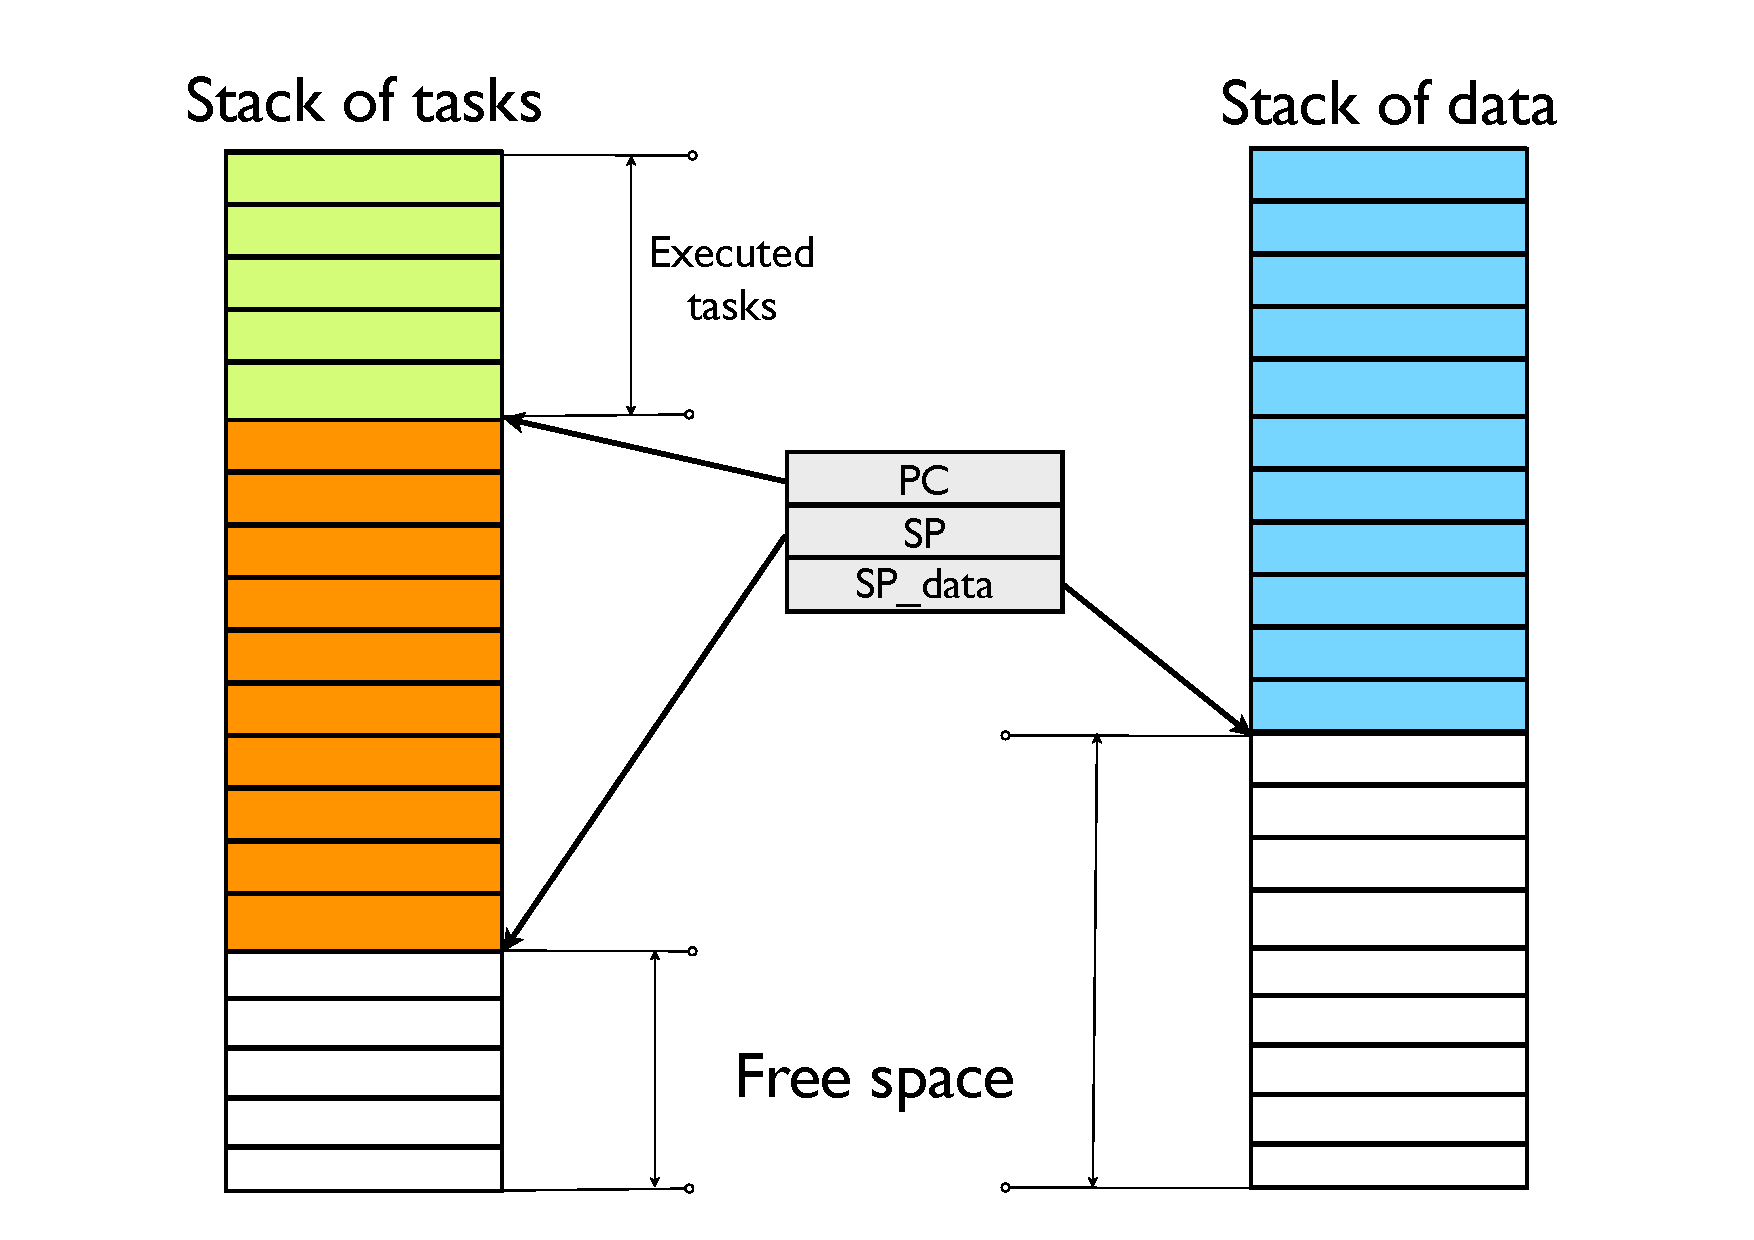
\includegraphics[width=0.5\linewidth]{stack}
\end{center}
\hrule
\caption{\kaapi stack: a dual stacks structure. At the left part of the figure, the stack of tasks with both \texttt{PC} (program counter) and \texttt{SP} pointer (stack pointer). At the right, the stack of data.}
\label{fig:stack}
\end{figure}

The algorithm to execute all tasks of a stack does not required recursion between task's bodies. 
\begin{figure}
\hrule
{\small
\begin{verbatim}
redo_work: 
  {
    if (task->body ==0) return 0;
    if (task->state == KAAPI_TASK_INIT) 
    { /* save stack pointers, pc is equal to task ! */
      saved_sp      = stack->sp;
      saved_sp_data = stack->sp_data;
      (*task->body)(task, stack);
      task->body = 0;
    
      /* push restore_frame task if newly created tasks */
      if (saved_sp < stack->sp) 
      { /* push retn task that will restore stack pointers 
           before executing the task 'task' */
        retn = kaapi_stack_top(stack);
        retn->body  = &kaapi_retn_body;
        /* next line is equiv to saving a frame. 
           retn->pdata must be equiv. to a kaapi_frame_t */
        retn->param.pdata[0] = task;   /* <=> save pc */
        retn->param.pdata[1] = saved_sp; 
        retn->param.pdata[2] = saved_sp_data;
        kaapi_stack_push(stack);

        /* update pc to the first forked task */
        task = stack->pc = saved_sp;
        goto redo_work;
      }
       
      task = ++stack->pc;
      goto redo_work;
    }
  }
  task = ++stack->pc;
  if (stack->pc >= stack->sp) return 0;
  goto redo_work;
}
\end{verbatim}
}
\hrule
\caption{Algorithm to execute tasks of a stack.}
\label{fig:stackalgo}
\end{figure}

\subsection{Task body}

The task body is a C-function that takes only two parameters:
\begin{description}
\item [kaapi\_task\_t*]: a pointer to the task to execute which also contains the list of parameters.
\item [kaapi\_stack\_t*]: the stack to store child  tasks created during execution of the task body.
\end{description}

When a task body returns, the \kaapi runtime test is child tasks have been created.
If it is the case, the runtime enqueue a special task (unstealable) which will restore the
context of the stack before execution the task body\footnote{This task is very similar to blr PowerPC instruction or ret/retn instruction in the X86 instructions set.}

The task body may wait on any POSIX synchronisation primitives (kaapi\_cond\_wait, kaapi\_ cond\_timedwait, kaapi\_mutex\_lock). In this case, the K-processor that executes the task, save the \kaapi stack context as well as the C-stack context in order to resume execution when synchronisation will be satisfied.

\subsection{Passing arguments} \label{sec:param}

A task may have at most \verb+KAAPI_TASK_MAX_DATA+ bytes for immediate parameters\footnote{This valuer is by default KAAPI\_TASK\_MAX\_DATA=32 bytes. A better value should be defined depending of average number of parameters for tasks}. These parameters could be viewed as integer (32 bits) or short (16 bits) or double (64 bits) or float (32 bits) or pointer (32 or 64 bits). All these parameters shared the same memory and not all these parameters must be used at the same time!

The name of parameters are the following.
\begin{itemize}
\item \verb+idata[0..KAAPI_TASK_MAX_IDATA-1]+: integer (32 bits) parameters.
\item \verb+sdata[0..KAAPI_TASK_MAX_SDATA-1]+: short (16 bits) parameters.
\item \verb+ddata[0..KAAPI_TASK_MAX_DDATA-1]+: double (64 bits) parameters.
\item \verb+fdata[0..KAAPI_TASK_MAX_FDATA-1]+: float (32 bits) parameters.
\item \verb+pdata[0..KAAPI_TASK_MAX_PDATA-1]+: pointer (32 or 64 bits depending on the OS/architecture) parameters.
\end{itemize}

The invariants maintained by the library are: integer parameters are 32 bits long; short are 16 bits long;  and the following equalities.
\begin{small}
$$
\begin{array}{ccc}
4 * KAAPI\_TASK\_MAX\_SDATA &   = & 2 * KAAPI\_TASK\_MAX\_IDATA \\
 & = & 2 * KAAPI\_TASK\_MAX\_FDATA \\
 & = &  KAAPI\_TASK\_MAX\_DDATA
\end{array}
$$
Due the variable size of pointer, we have:
$$ 
\begin{array}{ccc}
KAAPI\_TASK\_MAX\_PDATA &   = &  KAAPI\_TASK\_MAX\_DDATA \\
 & or &\\
2*KAAPI\_TASK\_MAX\_PDATA &   = &  KAAPI\_TASK\_MAX\_DDATA \\
\end{array}
$$
\end{small}

If a task has more parameters, then it should used the stack data to pass extra parameters. The following rules must be respected by all tasks. The purpose of these rules are to define exactly the location of parameters of a task given only the type
of each parameter.
\begin{itemize}
\item if all parameters of a task may be pass on immediate parameters then they should not be passed into the stack.
%The first parameter of type integer, short, double, float or pointer should used the free parameter data. The second parameter 
%of type integer, short, double, float or pointer is put on the next free parameter data. etc... If a parameter could not be store in 
%immediate parameters should be pass on the stack: then all the next parameter
\item if they are not enough immediate parameters, then pdata[{\small KAAPI\_TASK\_MAX\_PDATA-1}] is the pointer to the stack of data on the first parameter passed on the stack.
\end{itemize}
Note: some architecture / operating system defined such convention (parameter passing rule) between the caller and the callee. In theory, a task represents a function call, thus it should be necessary to adopt the same parameter passing rule.


\subsection{Shared objects}
A shared object allows to define a set of writers and readers that are synchronized through the produced value.
Two tasks that share a value through a shared object have been created together from a unique point in the past of the computation.This shared object is the classical shared object in Athapascan/Kaapi.\\

\new
In order to extend the kind of coordination between tasks that is permitted with \kaapi, we introduce a fifo shared object. Such object could be \textit{anonymous} and after its creation both the producers and consumers have to be forked with the fifo shared object as parameter. Producers and consumers not synchronized by a read / write dependency but by the availability of data into the fifo shared object. A consumer could only be started iff a value has been produced into the fifo shared object.

Nevertheless, we also introduce a \textit{named} fifo shared that could be defined by parallel tasks: two tasks without a priori any relationship could defined the fifo shared object given the same \textit{name}. \kaapi will manage the localisation of the producers and concumers in order to transport data from a task to an other.



\subsection{Access mode}

Each type should declare the access mode and type of each of its parameters. The access modes are the same than in Athapascan/Kaapi. Please refer to documentation about Athapascan to have a complete description of the semantic.
\begin{description}
\item [v]: the parameter is passed by value. A copy was made and the task may modify the copy without change the value of the effective parameter.
\item [r]: shared read access. The task may read the value of the shared object.
\item [rp]: shared read postponed access. The task may create a task that will read the value, but it cannot read itself the value.
\item [w]: shared write access. The task may write the value of the shared object. If the task do not write a value, then an undefined value is write to the shared value.
\item [wp]: shared write postponed access. The task may create a task that will write the value, but it cannot write itself the value.
\item [rw]: shared exclusive access. The task may read and write the value of the shared object.
\item [rwp]: shared exclusive postponed access. The task may create a task that will read or write the value, but it cannot read or write itself the value.
\item [cw]: shared concurrent write access. The task may accumulate a value of the shared object. The final value depend on the number of created task with concurrent write access.
\item [cwp]: shared concurrent write postponed access. The task may create a task that will accumulate a value, but it cannot accumulate itself a value.
\item [E]: is a special coding for empty mode, either because the access mode is unknown or has not yet be set.
%\item [fw]: shared fifo write access. The task may write a value to this kind of shared: the next value read from this shared will be the first write value produced with fw access mode.
\end{description}


\subsection{Fibonacci example}

Figure~\ref{fig:fibo} presents the code for Fibonacci example using the supid recursive code:
$$
fibo(n) = 
\left\{
\begin{array}{ll}
n & \mbox{if } n<2\\
fibo(n-1)+fibo(n-2) & \mbox{else}
\end{array}
\right.
$$
The calling convention used to create Fibonacci task is:
\begin{itemize}
\item \verb+idata[0]+: the input parameter $n$.
\item \verb+pdata[1]+: the pointer to the integer that store data computed by Fibo task.
\end{itemize}
Note that this code, could be easily generated by a compiler.

\begin{figure}[!h]
\hrule
\small
\begin{verbatim}
/* Fibonacci task body */
void fibo_body( kaapi_task_t* task, kaapi_stack_t* stack )
{
  if (task->idata[0] < 2)
  { /* store the input 'n' to the output value */
    *(int*)task->pdata[1] = task->idata[0];
  }
  else {
    int* result1 = (int*)kaapi_stack_pushshared(stack, sizeof(int));
    int* result2 = (int*)kaapi_stack_pushshared(stack, sizeof(int));

    kaapi_task_t* task1 = kaapi_stack_top(stack);
    task1->state    = KAAPI_TASK_INIT;
    task1->body     = &fibo_body;
    task1->idata[0] = task->idata[0]-1;
    task1->pdata[1] = result1;
    kaapi_stack_push(stack);

    kaapi_task_t* task2 = kaapi_stack_top(stack);
    task2->state    = KAAPI_TASK_INIT;
    task2->body     = &fibo_body;
    task2->idata[0] = task->idata[0]-2;
    task2->pdata[1] = result2;
    kaapi_stack_push(stack);

    kaapi_task_t* task_sum = kaapi_stack_top(stack);
    task_sum->state    = KAAPI_TASK_INIT;
    task_sum->body     = &sum_body;
    task_sum->pdata[0] = task->pdata[1];
    task_sum->pdata[1] = result1;
    task_sum->pdata[2] = result2;
    kaapi_stack_push(stack);    
 }
}
\end{verbatim}
\hrule
\caption{Classical Fibonacci example}
\label{fig:fibo}
\end{figure}
The access modes are defined by explicitly register the format of the task.
The figures~\ref{fig:stackfibo1} and~\ref{fig:stackfibo2} present a detailed of the content of the \kaapi stack.
\begin{figure}[!h]
\hrule
\hspace*{+12ex}
\begin{minipage}[t]{1\linewidth}
\begin{center}
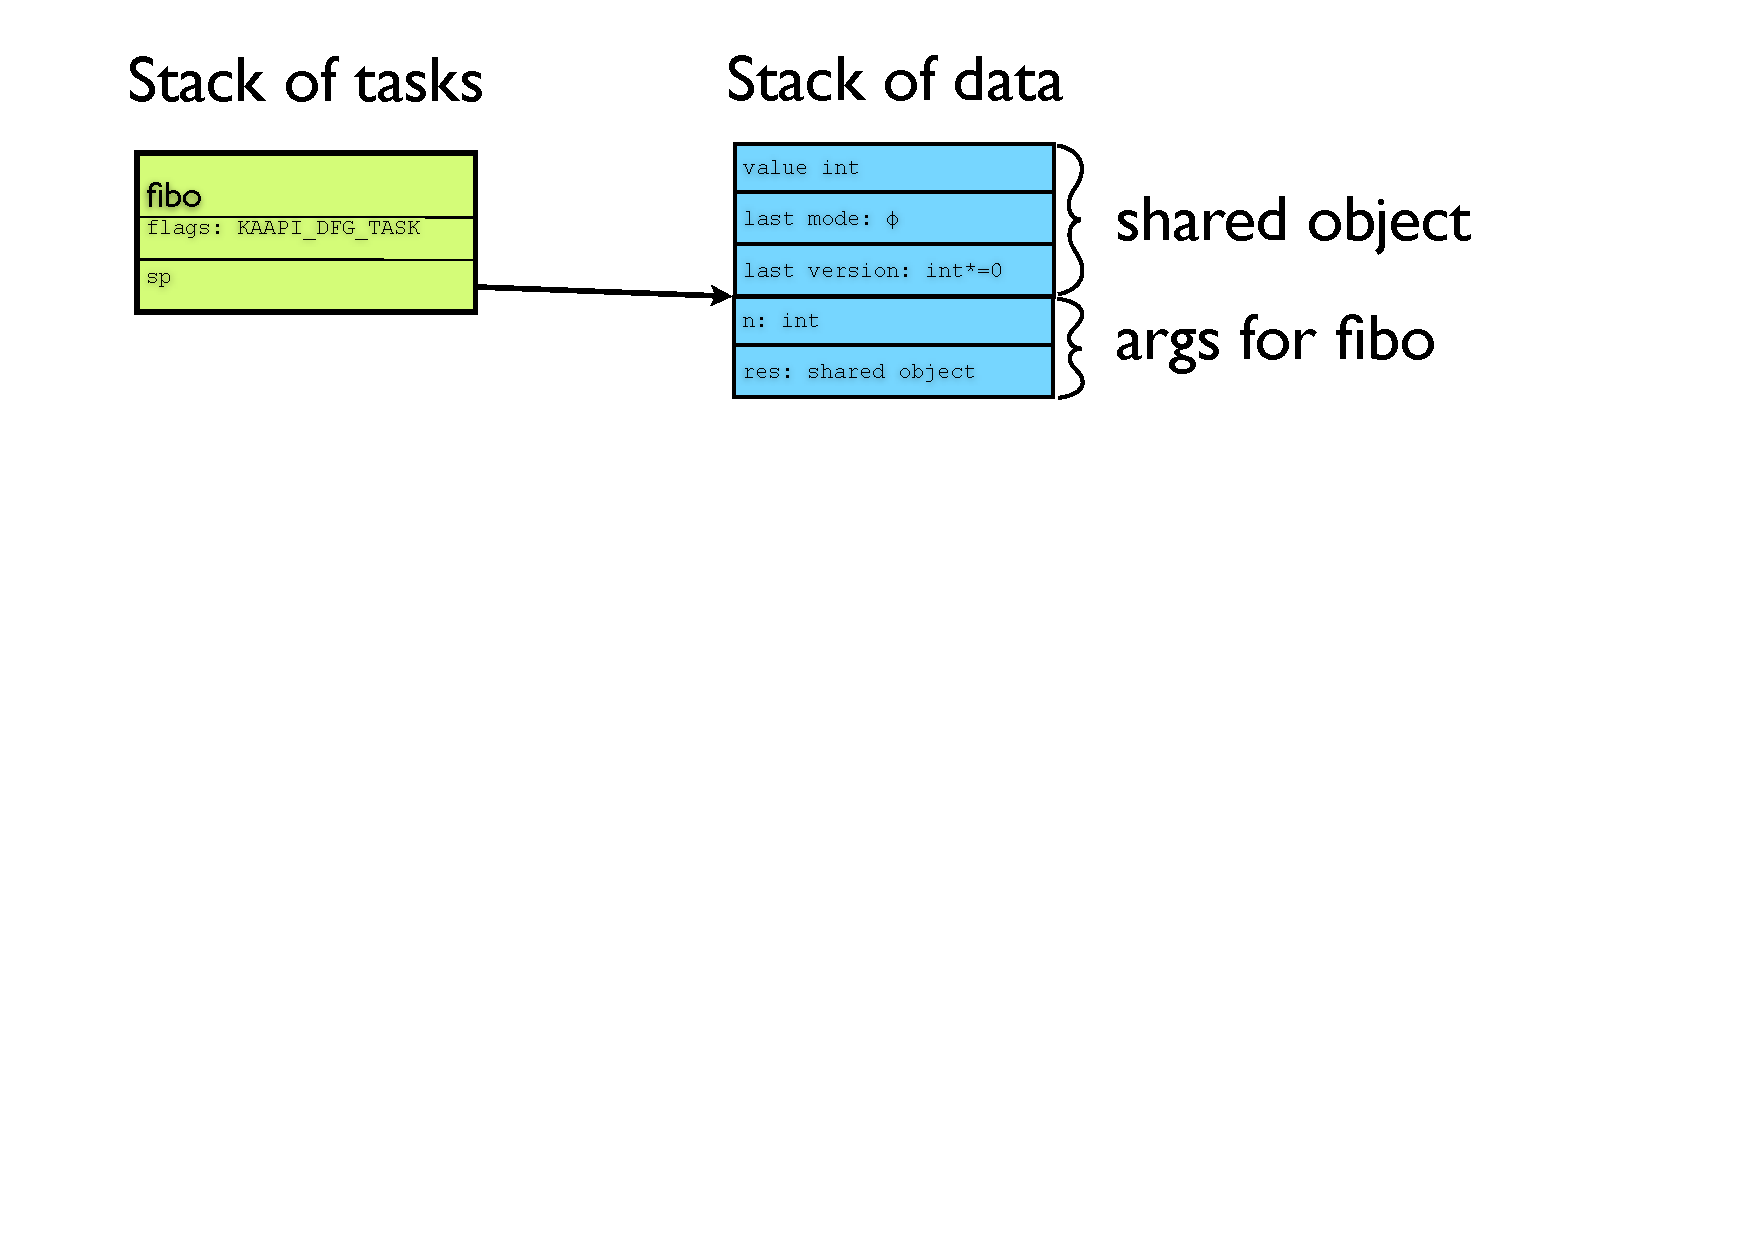
\includegraphics[width=1.0\linewidth]{stackfibo1}
\end{center}
\end{minipage}
\vspace*{-45ex}
\hrule
\caption{\kaapi stack before executing one instance of Fibonacci task. Task is pushed into the stack of tasks and the global data is pushed into the stack of data of the same \kaapi stack. Such construction is done during each recursive creation of Fibonacci task in the algorithm in figure~\ref{fig:fibo}.}
\label{fig:stackfibo1}
\end{figure}

\begin{figure}[!h]
\hrule
\hspace*{-5ex}
\begin{minipage}[t]{1\linewidth}
\begin{center}
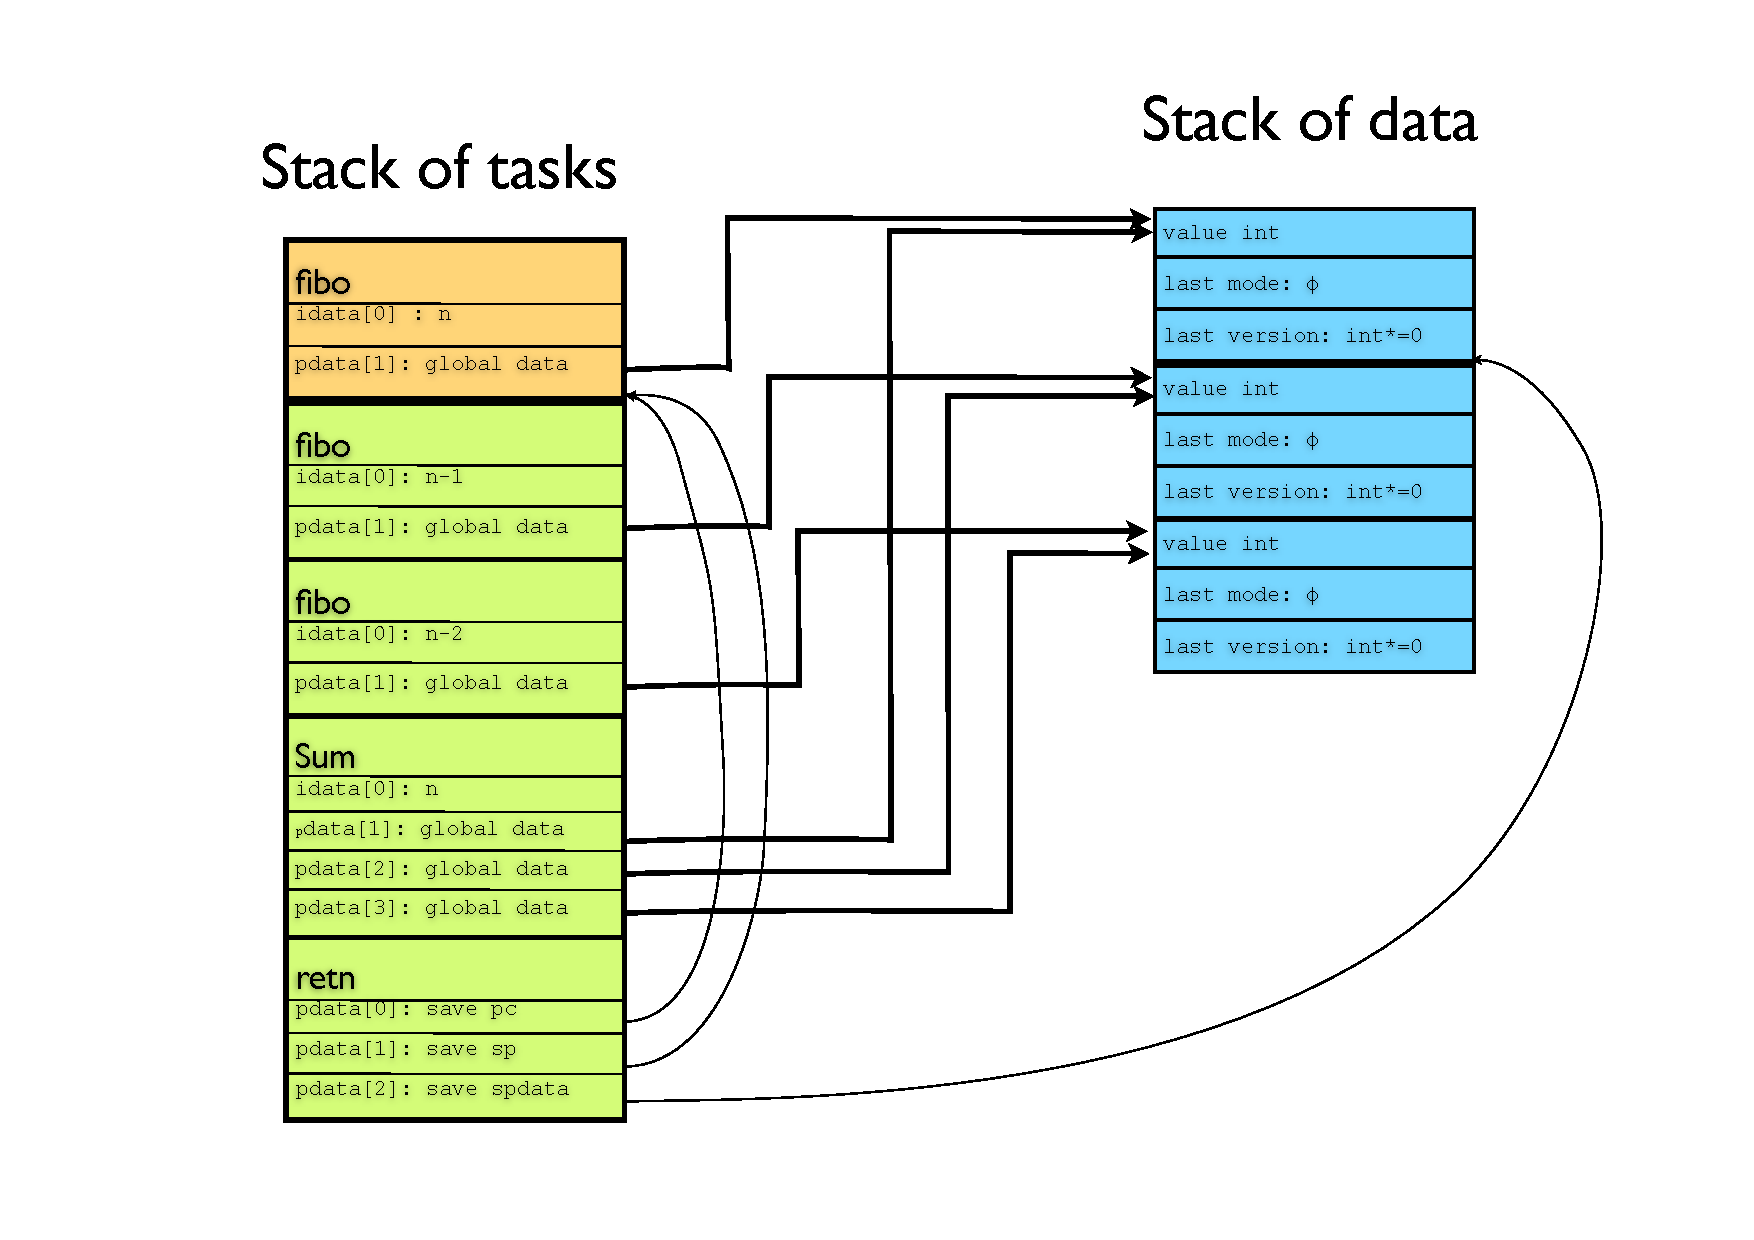
\includegraphics[width=1.0\linewidth]{stackfibo2}
\end{center}
\end{minipage}
\hrule
\caption{\kaapi stack after executing one instance of Fibonacci task of figure~\ref{fig:stackfibo1}.
The figure presents how accesses are represented. At the difference of the previous version of Kaapi,
the access to a same global data are not linked together, but they points to the same global data.
An other important difference: a task (retn) is added in order to restore stack pointers before executing the first (orange)  Fibonacci task.
}
\label{fig:stackfibo2}
\end{figure}


\newpage
\subsection{Data flow graph computation}
The purpose of this section is to present the new algorithm used in \kaapi to compute data flow constraints: \textit{i.e} how to compute the fact that a data is ready to be used in as parameter of task.

Some propositions are naturally deduced from the access mode and the semantic of Athapascan API.
\begin{proposition}
Let us consider a task $t$ with $k$ parameters. The following propositions are true: 
\begin{enumerate} \label{prop1}
\item \label{p1a} A task without parameters is always ready to execute.
\item \label{p1b} A effective parameter with access mode \textbf{[v]} is always ready to execute the task $t$.
\item \label{p1c} A effective parameter with access mode \textbf{[w]} or \textbf{[wp]} is always ready to execute the task $t$.
\item \label{p1d} A effective parameter with access mode \textbf{[r]} or \textbf{[rp]} is ready to execute the task $t$ iff the previous access(es) 
that write (\textbf{[w]}, \textbf{[wp]}, \textbf{[rw]}, \textbf{[rwp]}, \textbf{[cw]} or \textbf{[cwp]}) the value are parameters of tasks that have been already executed. 
\end{enumerate}
\end{proposition}

The following proposition also holds:
\begin{proposition}\label{prop2} 
The first task of a stack is always ready except iff its state is \textbf{KAAPI\_TASK\_INIT}.
\end{proposition}

Sequential execution of a \kaapi program, could be view as a repeated use of proposition~\ref{prop2}: the first task is created in state \textbf{KAAPI\_TASK\_INIT}, then it is ready. Thus it is executed and poped. The next task becomes the first of the stack.
\begin{proposition}
The sequential execution of a \kaapi program is to repeatedly execute the next task pointed by \texttt{pc} of the stack attached to the current flow of control using the algorithm~\ref{fig:stackalgo}.\\
No data flow constraints need to be computed.
\end{proposition}


\subsubsection{Representation of objets}

An access is an effective parameter of a task to a shared object.
An access to a shared object is a pointer to the global data and an optional range interval of values.
The global data stores a data, and the last version of the data and its access mode; these fields 
are only used by the work stealing algorithm to detect concurrent access.
The figure~\ref{fig:repobject} shows definitions of access and shared object.
\begin{figure}[!h]
\hrule
\small
\begin{verbatim}
struct kaapi_access_t  {
  kaapi_gd_t* gd;     /* global data that store value to use during
                         the execution of the task */
  /* optional value */
};

struct kaapi_access_steal_t  {
  void* data;         /* data to use during the execution of the task */
  /* optional value */
};

struct kaapi_gd_t {
  void*         data;         /* data used during normal execution */
  kaapi_amode_t last_mode;    /* access mode of the last version */
  void*         last_version; /* last version, used during work stealing */
};
\end{verbatim}
\hrule
\caption{Definition of access and shared object data structures}
\label{fig:repobject}
\end{figure}
In previous version of Kaapi, all accesses to the same shared object are linked together following the order of creation of the task. This chain of accesses was used to computed the readiness property of tasks. In the next sections, we propose an other algorithm that does not need to chain together accesses: it will improve both the memory usage of the graph representation as well as the overhead of $T_1$ versus $T_s$. The complexity of the algorithm that runs on each steal request remains equivalent.

\subsubsection{Execution by workstealing}
Using a work stealing algorithm will change the sequential execution: a thief may has stolen (a ready) task that will produce results read by next tasks in the execution order. At the instant of the work stealing decision to steal a task, the next tasks are probably not known. In order to avoid the computation of the data flow constraints before execution of each task, like in the first version of Athapascan, \kaapi is based on the following strategy:
\begin{enumerate}
\item The stolen task in the stack is marked as 'stolen'.
\item The algorithm~\ref{fig:stackalgo} executes tasks until the next task to execute is marked 'stolen'.
\end{enumerate}
Thus next tasks of a stolen task may have dependencies, the sequential execution is suspended and the thread begins to steal task from other threads, eventually from itself. 

Using such strategy, the data flow constraints are only computed during work stealing operations that are, in theory, not very many. This strategy was already implemented in Kaapi, the previous version of \kaapi.

\subsubsection{Computation of data flow constraints during work stealing operation}
The most important difference between Kaapi and \kaapi is that, in \kaapi the data flow graph representation is lighter: accesses to a shared object is not linked together; tasks in the stack are not linked together.
In order to detect ready task, the selection algorithm during work stealing operation uses \verb+last_XX+ data fields of the \verb+kaapi_gd_t+ data structure (see above, figure~\ref{fig:repobject}) to compute \textit{version} of a chain of accesses:
the selection algorithm iterates through all tasks in the stack, and then try to detect if all accesses of task is ready (and then the task will be ready to be stolen). The detection of readiness property of an access is done using the following rules:
\begin{itemize}
\item if the task is not executed (candidate task): let us note by \verb+m+ the access mode of the considered access and by \verb+(last_mode,+ \verb+last_version)+ the corresponding data fields of the associated \verb+kaapi_gd_t+ data structure.
\begin{itemize}
\item if $m$ is a postponed mode, then the access is ready. Then set \verb+last_+ \verb+mode+ to \verb+m+.
\item if $m$ is a write mode (\verb+w+ or \verb+cw+) then the access is ready. Then set \verb+last_+ \verb+mode+ to \verb+m+ 
and \verb+last_version+ to \verb+0+.
\item if $m$ is a read mode (\verb+r+) then the access is ready iff \verb+last_mode == E+ or \verb+last_mode+ \verb+== r+ and \verb+last_version !=0+ (the value has been produced). Then set \verb+last_+ \verb+mode+ to \verb+r+. The field \verb+last_version+ represent the data that will be read by the task.
\item if $m$ is a exclusive mode (\verb+rw+) then the access is ready iff \verb+last_mode == E+  and \verb+last_version !=0+ (the value has been produced). Then set \verb+last_+ \verb+mode+ to \verb+rw+. The field \verb+last_version+ represent the data that will be accessed by the task.
\end{itemize}
\item if the task was terminated (already stolen and marked as terminated), then:
\begin{itemize}
\item if $m$ is a write access, then set \verb+(last_mode,last_version)+ to \verb+(w, value_+ \verb+produced)+.
\item if $m$ is a read access, then set \verb+last_mode = r+
\item if $m$ is a exclusive access, then set \verb+(last_mode,last_version)+ to \verb+(rw, value_+ \verb+modified)+.
\end{itemize}
\end{itemize}



\subsection{Examples}


\begin{figure}
\hrule
\begin{verbatim}
uint16_t array_modes[] = { KAAPI_MODE_V, KAAPI_MODE_W };
kaapi_format_t array_formats[] = { KAAPI_INT, KAAPI_INT };

/* register the task format: a name, the body, the number of parameters
   and the access modes and types for each parameter.
   Not that the type of a shared (second parameter) is the type of 
   the value referenced by a shared.
*/
kaapi_register_taskformat(
                     "fibo",       /* the name */
                     &fibo_body,   /* the body */
                     2,            /* number of parameters */
                     array_modes,  /* access mode for each parameter */
                     array_formats /* type for each parameter */
); 
\end{verbatim}
\hrule
\caption{Definition of the format of a tasks}
\label{fig:fiboformat}
\end{figure}

\begin{figure}[!h]
\hrule
\begin{verbatim}
int main(int argc, char** argv)
{
  int err = 0;
  kaapi_stack_t* stack = kaapi_self_frame();

  int result = 0;
  
  /* t0 */
  double t0 = kaapi_get_elapsedtime();
  
  /* create the main task */
  kaapi_task_t* maintask = kaapi_stack_top(&stack);
  maintask->body  = &fibo_body;
  maintask->state = KAAPI_TASK_INIT;
  maintask->idata[0] = atoi(argv[1]);
  maintask->pdata[1] = &result;
  kaapi_stack_push(&stack);
  
  /* force execution of all tasks */
  kaapi_sync(&stack);
  /* here result contains the correct value */

  /*  t1 */
  double t1 = kaapi_get_elapsedtime();

  return 0;
}
\end{verbatim}
\hrule
\caption{Main function for Fibonacci example}
\label{fig:fibomain}
\end{figure}


\subsubsection{Transform example}

\subsubsection{Prefix example}

\section{Data flow graph representation}

\section{Work stealing algorithm}

%%%
%%%
%%%
\newpage
\chapter{API specification}

%%
%%
\section{Architecture model}

The target architecture for X-Kaapi is a grid of clusters of multi-core, many core nodes.
The architecture is assumed to hierarchically organized. At each level, all the cores use the same way to communicate together. The architecture is viewed as a non uniform memory architecture.
At the finer level of the hierarchy, each core has a private memory (L1 cache). The second level of cache  (L2), if exists, may be shared or not depending of the processor family / vendor. 

For each node, the main memory is assumed to be organized by memory banks with fast access for the core(s)'s owner. Other cores have an access through a high performance network (\textit{e.g.} idkoiff memory organization).

It is to the responsibility of the communication API (section~\ref{comapi}) to virtualize the memory organization in order to offer a common way to communicate. Nevertheless, the implementation should take care of the architecture to used to best method available.

%%
%%
\section{Execution model}
A program is composed of several threads of control into several process. 
Each process begins to execute the main entry point of the associated binary\footnote{It possible to have multiple binary, even if a SPMD model simply the complexity of the compilation / deployment stage.}. Each process is multithreaded and only the main thread  executes the initialization code before returning to the main user code. All processes have an unique identifier.

The initialization will create several worker threads that are called $k$-processors, and one $k$-processor pursues  the execution of main entry point of the process. It is called the main $k$-processor. All other $k$-processors begins by stealing work.

Each $k$-processor has two kinds of memory:
\begin{itemize}
\item A private memory that only the owner $k$-processor may access. This memory is associated to the C stack of function calls used by local computation done by the $k$-processor.
\item A write only shared memory that all $k$-processors could write but not read. This memory is used to put data structure shared between $k$-processors to implement the work stealing operations.
\item A shared memory that all other $k$-processors could read but not read. This memory allows read and write operations by all the $k$-processors and may be used to communicate user level data.
\end{itemize}
All the following API functions are designed such that communication due to the work stealing algorithm between threads use the write only shared memory in order to do remote write operation: a $k$-processor never read remote data during the work stealing operations.\\

\noindent\textbf{Note:} promotion between these kinds of memory have to be discussed.\\

\subsection{Memory operations ordering API}
We assumed that the memory read and write operation may be reordered by the compiler or the hardware. To enforce an ordering constraint on memory barrier we assume the availability of \textit{memory barrier}. Due to the unknown memory models of futurs target architectures of \kaapi, we assume two instructions to enforce reordering:
\begin{description}
\item [\texttt{kaapi\_write\_membarrier()}]: ensure that all  write operations prior to the barrier will have been committed to memory prior to any write following the barrier.
\item [\texttt{kaapi\_read\_membarrier()}]: ensure that all  read operations prior to the barrier will have been committed to memory prior to any read following the barrier.
\end{description}
Depending of the architecture, implementation of the functions may enforce a stronger ordering constraint that strictly required.


\section{Topology API}
\noindent{\bf People involved: }\\

The purpose of this API is to offers a view of the architecture. Libtopology\footnote{Renamed hwloc for hardware locality: http://www.open-mpi.org/projects/hwloc/} seems to be a complete API\footnote{The effectiveness use (simplicity, completeness of functions) of hwloc should be evaluated.}.

%%
%%
\section{Workstealing API}
\noindent{\bf People involved: }\\

This section describes all the functions required to create stealcontext structure and managing action at the different points of the work stealing algorithm.


\subsection{$k$-processor management}

Add the begining of the computation a certain number of $k$-processors are automatically created: the number of $k$-processors and their mapping on physical processors are controlled by environment variables defined in section~\ref{envvar}.

\subsection{Adding or deleting $k$-processors}
Nevertheless, it is possible to dynamically adjust the number of running $k$-processors of a process by setting the \textit{concurrency} of \kaapi. 
\begin{description}
\vspace*{3ex} \hrule width 4cm
\item [\texttt{int kaapi\_set\_concurrency(int concurrency)}]: change the current number of running $k$-processors to the new value $concurrency$. $concurrency$ is a non negative or null integer. If the old value is less or equal than the new value, then additional $(new\_value - old\_value)$ $k$-processors are created. Else $(old\_value - new\_value)$ $k$-processors are deleted.

Newly added $k$-processor begins to steal work from other $k$-processor. The $k$-processor is mapped onto the next free physical resource. This operation does not required any kind of synchronization.

Work or results owned by a deleted $k$-processor are attached to the closest alive $k$-processor following the hierarchy in order to minimize communication cost. In this case synchronization between deleted $k$-processor and the newly attached $k$-processor have a synchronization.

Return value is $0$ (KAAPI\_OK) in case of success else one of the following error code is returned:
\begin{description}
\item [KAAPI\_EINVAL]: invalid argument, typically passing $0$ or a negative value.
\item [KAAPI\_EGAIN]: the system lacked the necessary resources to create another $k$-processor.
\end{description}

\vspace*{3ex} \hrule width 4cm
\item [\texttt{int kaapi\_get\_concurrency(void)}]: return the current number of running $k$-processors.

\vspace*{3ex} \hrule width 4cm
\item [\texttt{kaapi\_processor\_t* kaapi\_self\_processor(void)}]: return a pointer to the current running $k$-processor.

\end{description}


\subsection{Posting a request}

\begin{description}
\vspace*{3ex} \hrule width 4cm
\item [\texttt{int kaapi\_request\_init( kaapi\_request\_t* kpr}]: initialize a new request data structure. This function must be called before any use of the request data.

Return value is $0$ (\texttt{KAAPI\_OK}) in case of success else one of the following error code is returned:
\begin{description}
\item [KAAPI\_EINVAL]: invalid argument, typically passing $0$ or invalid pointer.
\end{description}

\vspace*{3ex} \hrule width 4cm
\item [\texttt{int kaapi\_request\_destroy( kaapi\_request\_t* kpr}]: destroy an already initialized request data structure. After the call to the function, the request data cannot be used in any function.

Return value is $0$ (\texttt{KAAPI\_OK}) in case of success else one of the following error code is returned:
\begin{description}
\item [KAAPI\_EINVAL]: invalid argument, typically passing $0$ or invalid pointer.
\end{description}


\vspace*{3ex} \hrule width 4cm
\item [\texttt{int kaapi\_request\_post( kaapi\_processor\_t* thief}]~\\ \textbf{\texttt{kaapi\_processor\_t* victim, kaapi\_request\_t* kpsr )}}: the thief running $k$-processor post a steal request to the victim processor \verb+victim+. This is a non blocking call: in case of success, the running thief $k$-processor has to periodically check (\verb+kaapi_request_test+) or wait (\verb+kaapi_request_wait+) for the completion of the request.

Return value is $0$ (\texttt{KAAPI\_OK}) in case of success else one of the following error code is returned:
\begin{description}
\item [KAAPI\_EINVAL]: invalid argument, typically passing $0$ or invalid pointer.
\item [KAAPI\_EBUSY]: the victim processor does not accept request.
\end{description}


\vspace*{3ex} \hrule width 4cm
\item [\texttt{int kaapi\_request\_test(  kaapi\_request\_t* kpsr )}:] return 0 if the request has been processed, else return one of the follwing error code.
On successful return, the status a call to \verb+kaapi_request_status+ allows to return the status the request.
\begin{description}
\item [KAAPI\_EINVAL]: invalid argument, typically passing $0$ or invalid pointer.
\item [KAAPI\_EINPROGRESS]: the request is not yet processed.
\item [KAAPI\_EINTR]: the processing of request has been interrupt, may due terminaison.
\end{description}

\vspace*{3ex} \hrule width 4cm
\item [\texttt{int kaapi\_request\_wait(  kaapi\_request\_t* kpsr )}:] return 0 if the request has been processed, else return one of the follwing error code.
On successful return, the status a call to \verb+kaapi_request_status+ allows to return the status the request.
\begin{description}
\item [KAAPI\_EINVAL]: invalid argument, typically passing $0$ or invalid pointer.
\item [KAAPI\_EINTR]: the processing of request has been interrupt, may due terminaison.
\end{description}


\vspace*{3ex} \hrule width 4cm 
\item [\texttt{int kaapi\_request\_status(  kaapi\_request\_t* kpsr )}:] return the status of the request using the following code
\begin{description}
\item [KAAPI\_OK]: the request has successful steal work.
\item [KAAPI\_EAGAIN]: the request does not steal work and it could be reposted to other $k$-processor.
\item [KAAPI\_EINTR]: the processing of request has been interrupt, may due terminaison.
\item [KAAPI\_EINVAL]: invalid argument, typically passing $0$ or invalid pointer.
\end{description}

\vspace*{3ex} \hrule width 4cm 
\item [\texttt{int kaapi\_request\_cancel(  kaapi\_request\_t* kpsr )}:] cancel a request posted to a $k$-processor. 
If successful,  the \verb+kaapi_request_cancel+ function will return zero.  Otherwise, an error number will be returned to indicate the error.

\inote{This function is generally difficult to implement. The victim processor may have already stored the reply while the thief is trying to cancel the request. If the protocol to ensure consistency required a strong synchronization in every reply, then this function may be suppressed from the API. }

\begin{description}
\item [KAAPI\_OK]: the request has been successfully canceled.
\item [KAAPI\_EBUSY]: the request has been already replied with a result. 

A call to \verb+ kaapi_request_status+ function will return its status .
\item [KAAPI\_EINVAL]: invalid argument, typically passing $0$ or invalid pointer.
\end{description}

\end{description}


\subsection{Access to user defined arguments of a request}
A request data structure contains a buffer of \verb+KAAPI_REQUEST_DATA_SIZE+ bytes (at least 16 bytes) that could be used to store user defined arguments. The data structure \verb+kaapi_request_t+ contains an opaque field that points to the first byte of this buffer.

\inote{Does the size of buffer should be bigger ? Does the buffer size should dynamic ? }

In order to read or write this data, the following functions should be used:
\begin{description}
\vspace*{3ex} \hrule width 4cm
\item [\texttt{int kaapi\_request\_writedata(kaapi\_request\_t* kpr, }]~\\
\textbf{\texttt{int count, const void* src)}}: 
write \verb+count+ bytes from \verb+src+ to the internal request buffer.
Upon successful completion the number of bytes which were written is returned (non negative integer).
If a negative integer is return then the absolute value indicate the error:
\begin{description}
\item [KAAPI\_EINVAL]: invalid argument, typically passing $0$ or a negative value.
\item [KAAPI\_ENOMEM]: the request lacked the necessary resources to store count byte.
\end{description}

\vspace*{3ex} \hrule width 4cm
\item [\texttt{int kaapi\_request\_readdata(kaapi\_request\_t* kpr, }]~\\
\textbf{\texttt{int count, void* dest)}}: 
read \verb+count+ bytes from the internal request buffer to \verb+kpr+.
Upon successful completion the number of bytes which were read is returned (non negative integer).
If a negative integer is return then the absolute value indicate the error:
\begin{description}
\item [KAAPI\_EINVAL]: invalid argument, typically passing $0$ or a negative value.
\item [KAAPI\_ENOMEM]: the request lacked the necessary resources to store count byte.
\end{description}


\vspace*{3ex} \hrule width 4cm
\item [\texttt{const void* kaapi\_request\_data(kaapi\_request\_t* kpr)}]
This function may only by called by the owner of the request (the thread that initialized it).
Upon successful completion a pointer to the first byte of the internal buffer is returned. Else it returns 0.
\begin{description}
\item [0]: invalid argument, typically passing $0$ or a negative value, or the request pointer is not owned by the caller
\end{description}
\inote{Testing if the request is owned by the caller thread may required extra informations that are not required for normal execution. This extra informations/code should be available during debugging compilation mode. Thus the value retuned by the function may has to be defined as 'undefined' is the call does not occur with the context of the owner...}
\end{description}



\subsection{Selection of victim $k$-processor}




\section{StealContext}

\paragraph{Pushing and poping a StealContext structure}

\paragraph{Cooperative processing of steal request}

\paragraph{Concurrent processing of steal request}

\paragraph{Finalization point}

\paragraph{Preemption and preemption point}

\paragraph{StealContext data structure}

\section{Implementation}

In order to avoid most of dynamic memory management, the maximal set of $k$-processors per process is bounded by a constant \verb+KAAPI_MAX_KPROCESSORS+ which at least the number of physical cores on the machine.
Each $k$-processor has an unique local (process wide) identifier in $[0, KAAPI\_MAX\_KPROCESSORS-1]$.

\subsection{\texttt{kaapi\_processor\_t} data structure}

Each $k$-processors have a \verb+KAAPI_MAX_KPROCESSORS+ array of requests that posted by other $k$-processors.
If the entry $i$ is non null, then the $k$-processor with local identifier $i$ has posted a request. Moreover, each $k$-processor has a flag indicating if at least one request has been posted. The structure \texttt{kaapi\_processor\_t} has at least the following definition of fields:
\begin{verbatim}
struct kaapi_processor_t {
  unsigned int     _localid;
  kaapi_request_t* _request[KAAPI_MAX_KPROCESSORS]; 
  int              _flag; /* 0 or 1 */
};
\end{verbatim}

\subsection{\texttt{kaapi\_request\_t} data structure}


\subsection{Algorithm to post a request}
The algorithm to post a request is the following\footnote{Not that the current implementation is not this one: in place of set to 1 the flag on the victim, an atomic increment is executed on the flag.}:
\begin{verbatim}
1.  int kaapi request post( 
2.          kaapi processor t* thief, 
3.          kaapi processor t* victim, 
4.          kaapi request t* kpr )
5.  {
6.    kpr->_state = KAAPI_REQUEST_POSTED ;
7.    kaapi_write_membarrier();
8.    victim->_request[ thief->_localid ] = kpr ;
9.    victim->_flag = 1;
10. }
\end{verbatim}
Line 7 is required memory barrier to ensure that previous write operations will be view prior to write operations following the barrier : If the victim $k$-processor views the request (line 8 committed to the memory), then the request data will also be viewed in a coherent state.

\subsection{Management of data}


%%
%%
\section{Threads and synchronizations API}
\noindent{\bf People involved: }\\

\subsection{Thread creation}

\begin{description}
\vspace*{3ex} \hrule width 4cm
\item [\texttt{int kaapi\_create(kaapi\_t* \_\_restrict thread, const kaapi\_attr\_t* \_\_restrict attr,}]~\\
\textbf{\texttt{void*(*start\_routine)(void *), void* \_\_restrict arg)}} :

create a thread that may be a system thread (\verb+KAAPI_SYSTEM_SCOPE+ or
\verb+KAAPI_PROCESSOR_SCOPE+) or a user thread (\verb+KAAPI_PROCESS_SCOPE+).
After this call, the thread descriptor \verb+thread+ is allocated For system
threads, a thread is created with \verb+kaapi_start_system_handler+ as
starting function.  For user threads, a thread is also created but with
\verb+kaapi_start_process_handler+ as starting function.

If successful, the kaapi\_create() function shall return zero; otherwise, an
error number shall be returned to indicate the error.

The kaapi\_create() function shall fail if:

\begin{description}
\item [KAAPI\_EAGAIN]: The system lacked the necessary resources to create
  another thread, or the system-imposed limit on the total number of threads
  in a process {PTHREAD\_THREADS\_MAX} would be exceeded.
\item [KAAPI\_EPERM]: The caller does not have appropriate permission to set
  the required scheduling parameters or scheduling policy.
\item [KAAPI\_EINVAL]: The attributes specified by attr are invalid.
\end{description}

\end{description}

\verb+kaapi_start_system_handler+ as starting function.
\verb+kaapi_start_process_handler+ as starting function.



\subsection{Mutex}

%%%%%%%%%%%%%%%%%%%%%%%%%%%%%%%%%%%%%%%%%%%%%%%%%%%%%%%%%%%%%%%%%%%%%%%%%%%%%%
% MUTEX ATTRIBUTES
%%%%%%%%%%%%%%%%%%%%%%%%%%%%%%%%%%%%%%%%%%%%%%%%%%%%%%%%%%%%%%%%%%%%%%%%%%%%%%
\begin{description}
\vspace*{3ex} \hrule width 4cm
\vspace*{3ex} 
\item [\texttt{int kaapi\_mutexattr\_init (kaapi\_mutexattr\_t *attr)}]
\item [\texttt{int kaapi\_mutexattr\_destroy (kaapi\_mutexattr\_t *attr)}]~\\
%\textbf{\texttt{int kaapi\_mutexattr\_destroy (kaapi\_mutexattr\_t *attr)}} :

The kaapi\_mutexattr\_destroy() function shall destroy a mutex attributes
object. A destroyed attr attributes object can be reinitialized using
kaapi\_mutexattr\_init(); the results of otherwise referencing the object
after it has been destroyed are undefined.

The kaapi\_mutexattr\_init() function shall initialize a mutex attributes
object attr with the default value for all of the attributes defined by the
implementation.

Results are undefined if kaapi\_mutexattr\_init() is called specifying an
already initialized attr attributes object.

After a mutex attributes object has been used to initialize one or more
mutexes, any function affecting the attributes object (including destruction)
shall not affect any previously initialized mutexes.

Upon successful completion, kaapi\_mutexattr\_destroy() and
kaapi\_mutexattr\_init() shall return zero; otherwise, an error number shall
be returned to indicate the error.

The kaapi\_mutexattr\_destroy() function may fail if:

\begin{description}
\item [KAAPI\_EINVAL]: The value specified by attr is invalid.
\end{description}

The kaapi\_mutexattr\_init() function shall not fail.

These functions shall not return an error code of \verb+KAAPI_ENOMEM+.
\end{description}

%%%%%%%%%%%%%%%%%%%%%%%%%%%%%%%%%%%%%%%%%%%%%%%%%%%%%%%%%%%%%%%%%%%%%%%%%%%%%%

\begin{description}
\vspace*{3ex} \hrule width 4cm
\vspace*{3ex} 
\item [\texttt{int kaapi\_mutexattr\_gettype (const kaapi\_mutexattr\_t
    *\_\_restrict, int *\_\_restrict)}]
\item [\texttt{int kaapi\_mutexattr\_settype (kaapi\_mutexattr\_t *, int)}]~\\

The kaapi\_mutexattr\_gettype() and kaapi\_mutexattr\_settype() functions,
respectively, shall get and set the mutex type attribute. This attribute is
set in the type parameter to these functions. The default value of the type
attribute is KAAPI\_MUTEX\_NORMAL.

The type of mutex is contained in the type attribute of the mutex attributes.

The type of mutex is contained in the type attribute of the mutex
attributes. Valid mutex types include:

KAAPI\_MUTEX\_NORMAL: This type of mutex does not detect deadlock. A thread
attempting to relock this mutex without first unlocking it shall
deadlock. Attempting to unlock a mutex locked by a different thread results in
undefined behavior. Attempting to unlock an unlocked mutex results in
undefined behavior.

KAAPI\_MUTEX\_RECURSIVE: A thread attempting to relock this mutex without
first unlocking it shall succeed in locking the mutex. Multiple locks of this
mutex shall require the same number of unlocks to release the mutex before
another thread can acquire the mutex. A thread attempting to unlock a mutex
which another thread has locked shall return with an error. A thread
attempting to unlock an unlocked mutex shall return with an error.

Upon successful completion, the kaapi\_mutexattr\_gettype() function shall
return zero and store the value of the type attribute of attr into the object
referenced by the type parameter. Otherwise, an error shall be returned to
indicate the error.

If successful, the kaapi\_mutexattr\_settype() function shall return zero;
otherwise, an error number shall be returned to indicate the error.

The kaapi\_mutexattr\_settype() function shall fail if:

\begin{description}
\item [KAAPI\_EINVAL]: The value type is invalid.
\end{description}

The kaapi\_mutexattr\_gettype() and kaapi\_mutexattr\_settype() functions may
fail if:

\begin{description}
\item [KAAPI\_EINVAL]: The value specified by attr is invalid.
\end{description}
\end{description}

%% Mutex Attributes Not Implemented here?

%%%%%%%%%%%%%%%%%%%%%%%%%%%%%%%%%%%%%%%%%%%%%%%%%%%%%%%%%%%%%%%%%%%%%%%%%%%%%%
% MUTEX MANAGEMENT
%%%%%%%%%%%%%%%%%%%%%%%%%%%%%%%%%%%%%%%%%%%%%%%%%%%%%%%%%%%%%%%%%%%%%%%%%%%%%%

\begin{description}
\vspace*{3ex} \hrule width 4cm
\vspace*{3ex} 
\item [\texttt{int kaapi\_mutex\_init (kaapi\_mutex\_t *\_\_restrict mutex,}]~\\
\textbf{\texttt{ const kaapi\_mutexattr\_t *\_\_restrict attr)}}
\item [\texttt{int kaapi\_mutex\_destroy (kaapi\_mutex\_t *mutex)}]~\\
%\textbf{\texttt{int kaapi\_mutexattr\_destroy (kaapi\_mutexattr\_t *attr)}} :

The kaapi\_mutex\_destroy() function shall destroy the mutex object referenced
by mutex; the mutex object becomes, in effect, uninitialized. An
implementation may cause kaapi\_mutex\_destroy() to set the object referenced
by mutex to an invalid value. A destroyed mutex object can be reinitialized
using kaapi\_mutex\_init(); the results of otherwise referencing the object
after it has been destroyed are undefined.

It shall be safe to destroy an initialized mutex that is unlocked. Attempting
to destroy a locked mutex results in undefined behavior.

The kaapi\_mutex\_init() function shall initialize the mutex referenced by
mutex with attributes specified by attr. If attr is NULL, the default mutex
attributes are used; the effect shall be the same as passing the address of a
default mutex attributes object. Upon successful initialization, the state of
the mutex becomes initialized and unlocked.

Only mutex itself may be used for performing synchronization. The result of
referring to copies of mutex in calls to kaapi\_mutex\_lock(),
kaapi\_mutex\_trylock(), kaapi\_mutex\_unlock(), and kaapi\_mutex\_destroy()
is undefined.

Attempting to initialize an already initialized mutex results in undefined
behavior.

In cases where default mutex attributes are appropriate, the macro
KAAPI\_MUTEX\_INITIALIZER can be used to initialize mutexes that are
statically allocated. The effect shall be equivalent to dynamic initialization
by a call to kaapi\_mutex\_init() with parameter attr specified as NULL,
except that no error checks are performed.

If successful, the kaapi\_mutex\_destroy() and kaapi\_mutex\_init() functions
shall return zero; otherwise, an error number shall be returned to indicate
the error.

The kaapi\_mutex\_destroy() function may fail if:

\begin{description}
\item [KAAPI\_EBUSY]: The implementation has detected an attempt to destroy
  the object referenced by mutex while it is locked or referenced (for
  example, while being used in a kaapi\_cond\_timedwait() or
  kaapi\_cond\_wait()) by another thread.
\item [KAAPI\_EINVAL]: The value specified by mutex is invalid.
\end{description}

The kaapi\_mutex\_init() function shall fail if:

\begin{description}
\item [KAAPI\_EAGAIN]: The system lacked the necessary resources (other than
  memory) to initialize another mutex.
\item [KAAPI\_ENOMEM]: Insufficient memory exists to initialize the mutex.
\item [KAAPI\_EPERM]: The caller does not have the privilege to perform the
  operation.
\end{description}

The kaapi\_mutex\_init() function may fail if:

\begin{description}
\item [KAAPI\_EBUSY]: The implementation has detected an attempt to
  reinitialize the object referenced by mutex, a previously initialized, but
  not yet destroyed, mutex.
\item [KAAPI\_EINVAL]: The value specified by attr is invalid.
\end{description}
\end{description}

%%%%%%%%%%%%%%%%%%%%%%%%%%%%%%%%%%%%%%%%%%%%%%%%%%%%%%%%%%%%%%%%%%%%%%%%%%%%%%

\begin{description}
\vspace*{3ex} \hrule width 4cm
\vspace*{3ex} 
\item [\texttt{int kaapi\_mutex\_lock (kaapi\_mutex\_t *mutex)}]
\item [\texttt{int kaapi\_mutex\_trylock (kaapi\_mutex\_t *mutex)}]
\item [\texttt{int kaapi\_mutex\_unlock (kaapi\_mutex\_t *mutex)}]~\\
%\textbf{\texttt{int kaapi\_mutexattr\_destroy (kaapi\_mutexattr\_t *attr)}} :

The mutex object referenced by mutex shall be locked by calling
kaapi\_mutex\_lock(). If the mutex is already locked, the calling thread shall
block until the mutex becomes available. This operation shall return with the
mutex object referenced by mutex in the locked state with the calling thread
as its owner.

[XSI] [Option Start] If the mutex type is KAAPI\_MUTEX\_NORMAL, deadlock
detection shall not be provided. Attempting to relock the mutex causes
deadlock. If a thread attempts to unlock a mutex that it has not locked or a
mutex which is unlocked, undefined behavior results.

If the mutex type is KAAPI\_MUTEX\_ERRORCHECK, then error checking shall be
provided. If a thread attempts to relock a mutex that it has already locked,
an error shall be returned. If a thread attempts to unlock a mutex that it has
not locked or a mutex which is unlocked, an error shall be returned.

If the mutex type is KAAPI\_MUTEX\_RECURSIVE, then the mutex shall maintain
the concept of a lock count. When a thread successfully acquires a mutex for
the first time, the lock count shall be set to one. Every time a thread
relocks this mutex, the lock count shall be incremented by one. Each time the
thread unlocks the mutex, the lock count shall be decremented by one. When the
lock count reaches zero, the mutex shall become available for other threads to
acquire. If a thread attempts to unlock a mutex that it has not locked or a
mutex which is unlocked, an error shall be returned.

If the mutex type is KAAPI\_MUTEX\_DEFAULT, attempting to recursively lock the
mutex results in undefined behavior. Attempting to unlock the mutex if it was
not locked by the calling thread results in undefined behavior. Attempting to
unlock the mutex if it is not locked results in undefined behavior. [Option
  End]

The kaapi\_mutex\_trylock() function shall be equivalent to
kaapi\_mutex\_lock(), except that if the mutex object referenced by mutex is
currently locked (by any thread, including the current thread), the call shall
return immediately. If the mutex type is KAAPI\_MUTEX\_RECURSIVE and the mutex
is currently owned by the calling thread, the mutex lock count shall be
incremented by one and the kaapi\_mutex\_trylock() function shall immediately
return success.

The kaapi\_mutex\_unlock() function shall release the mutex object referenced
by mutex. [XSI] [Option Start] The manner in which a mutex is released is
dependent upon the mutex's type attribute. [Option End] If there are threads
blocked on the mutex object referenced by mutex when kaapi\_mutex\_unlock() is
called, resulting in the mutex becoming available, the scheduling policy shall
determine which thread shall acquire the mutex.

[XSI] [Option Start] (In the case of KAAPI\_MUTEX\_RECURSIVE mutexes, the
mutex shall become available when the count reaches zero and the calling
thread no longer has any locks on this mutex.) [Option End]

If a signal is delivered to a thread waiting for a mutex, upon return from the
signal handler the thread shall resume waiting for the mutex as if it was not
interrupted.

If successful, the kaapi\_mutex\_lock() and kaapi\_mutex\_unlock() functions
shall return zero; otherwise, an error number shall be returned to indicate
the error.

The kaapi\_mutex\_trylock() function shall return zero if a lock on the mutex
object referenced by mutex is acquired. Otherwise, an error number is returned
to indicate the error.

The kaapi\_mutex\_lock() and kaapi\_mutex\_trylock() functions shall fail if:

\begin{description}
\item [KAAPI\_EINVAL]: The mutex was created with the protocol attribute
  having the value KAAPI\_PRIO\_PROTECT and the calling thread's priority is
  higher than the mutex's current priority ceiling.
\end{description}

The kaapi\_mutex\_trylock() function shall fail if:

\begin{description}
\item [KAAPI\_EBUSY]: The mutex could not be acquired because it was already
  locked.
\end{description}

The kaapi\_mutex\_lock(), kaapi\_mutex\_trylock(), and kaapi\_mutex\_unlock()
functions may fail if:

\begin{description}
\item [KAAPI\_EINVAL]: The value specified by mutex does not refer to an
  initialized mutex object.
\item [KAAPI\_EAGAIN]: [XSI] [Option Start] The mutex could not be acquired
  because the maximum number of recursive locks for mutex has been
  exceeded. [Option End]
\end{description}

The kaapi\_mutex\_lock() function may fail if:

\begin{description}
\item [KAAPI\_EDEADLK]: A deadlock condition was detected or the current
  thread already owns the mutex.
\end{description}

The kaapi\_mutex\_unlock() function may fail if:

\begin{description}
\item [KAAPI\_EPERM]
    The current thread does not own the mutex. 
\end{description}
\end{description}


\subsection{Condition}

%%%%%%%%%%%%%%%%%%%%%%%%%%%%%%%%%%%%%%%%%%%%%%%%%%%%%%%%%%%%%%%%%%%%%%%%%%%%%%
% CONDITION
%%%%%%%%%%%%%%%%%%%%%%%%%%%%%%%%%%%%%%%%%%%%%%%%%%%%%%%%%%%%%%%%%%%%%%%%%%%%%%
Our conditions are implemented same way as POSIX conditions are blablabla. We
do not currently implement the following function :

\begin{verbatim}
int   kaapi_condattr_getclock(const kaapi_condattr_t *restrict,
          clockid_t *restrict);

int   kaapi_condattr_getpshared(const kaapi_condattr_t *restrict,
          int *restrict);

int   kaapi_condattr_setclock(kaapi_condattr_t *, clockid_t);

int   kaapi_condattr_setpshared(kaapi_condattr_t *, int);
\end{verbatim}

%%%%%%%%%%%%%%%%%%%%%%%%%%%%%%%%%%%%%%%%%%%%%%%%%%%%%%%%%%%%%%%%%%%%%%%%%%%%%%

%% \begin{description}
%% \vspace*{3ex} \hrule width 4cm
%% \vspace*{3ex} 
%% \item [\texttt{}]
%% \item [\texttt{}]~\\

%% \paragraph{Description}~\\
%% Texte

%% \paragraph{Return Value}~\\
%% Texte

%% \paragraph{Errors}~\\
%% Texte

%% \begin{description}
%% \item [KAAPI\_EINVAL]: 
%% \end{description}

%% \end{description}

%%%%%%%%%%%%%%%%%%%%%%%%%%%%%%%%%%%%%%%%%%%%%%%%%%%%%%%%%%%%%%%%%%%%%%%%%%%%%%

\begin{description}
\vspace*{3ex} \hrule width 4cm
\vspace*{3ex} 
\item [\texttt{int kaapi\_cond\_broadcast(kaapi\_cond\_t *cond);}]
\item [\texttt{int kaapi\_cond\_signal(kaapi\_cond\_t *cond);}]~\\

\paragraph{Description}~\\
These functions shall unblock threads blocked on a condition variable.

The kaapi\_cond\_broadcast() function shall unblock all threads currently
blocked on the specified condition variable cond.

The kaapi\_cond\_signal() function shall unblock at least one of the threads
that are blocked on the specified condition variable cond (if any threads are
blocked on cond).

If more than one thread is blocked on a condition variable, the scheduling
policy shall determine the order in which threads are unblocked. When each
thread unblocked as a result of a kaapi\_cond\_broadcast() or
kaapi\_cond\_signal() returns from its call to kaapi\_cond\_wait() or
kaapi\_cond\_timedwait(), the thread shall own the mutex with which it called
kaapi\_cond\_wait() or kaapi\_cond\_timedwait(). The thread(s) that are
unblocked shall contend for the mutex according to the scheduling policy (if
applicable), and as if each had called kaapi\_mutex\_lock().

The kaapi\_cond\_broadcast() or kaapi\_cond\_signal() functions may be called
by a thread whether or not it currently owns the mutex that threads calling
kaapi\_cond\_wait() or kaapi\_cond\_timedwait() have associated with the
condition variable during their waits; however, if predictable scheduling
behavior is required, then that mutex shall be locked by the thread calling
kaapi\_cond\_broadcast() or kaapi\_cond\_signal().

The kaapi\_cond\_broadcast() and kaapi\_cond\_signal() functions shall have no
effect if there are no threads currently blocked on cond.

The behavior is undefined if the value specified by the cond argument to
kaapi\_cond\_broadcast() or kaapi\_cond\_signal() does not refer to an
initialized condition variable.

\paragraph{Return Value}~\\
If successful, the kaapi\_cond\_broadcast() and kaapi\_cond\_signal()
functions shall return zero; otherwise, an error number shall be returned to
indicate the error.

\paragraph{Errors}~\\
These functions shall not return an error code of [KAAPI\_EINTR].

\end{description}

%%%%%%%%%%%%%%%%%%%%%%%%%%%%%%%%%%%%%%%%%%%%%%%%%%%%%%%%%%%%%%%%%%%%%%%%%%%%%%

\begin{description}
\vspace*{3ex} \hrule width 4cm
\vspace*{3ex} 
\item [\texttt{ int kaapi\_cond\_destroy(kaapi\_cond\_t *cond);}]
\item [\texttt{ int kaapi\_cond\_init(kaapi\_cond\_t *restrict cond,}]~\\
\textbf{\texttt{ const kaapi\_condattr\_t *restrict attr);}}
\item [\texttt{ kaapi\_cond\_t cond = KAAPI\_COND\_INITIALIZER;}]~\\

\paragraph{Description}~\\
Texte

\paragraph{Return Value}~\\
Texte

\paragraph{Errors}~\\
Texte

\begin{description}
\item [KAAPI\_EINVAL]: 
\end{description}

\end{description}

%%%%%%%%%%%%%%%%%%%%%%%%%%%%%%%%%%%%%%%%%%%%%%%%%%%%%%%%%%%%%%%%%%%%%%%%%%%%%%

\begin{description}
\vspace*{3ex} \hrule width 4cm
\vspace*{3ex} 
\item [\texttt{int kaapi\_cond\_timedwait(kaapi\_cond\_t *restrict cond,}]~\\
\textbf{\texttt{kaapi\_mutex\_t *restrict mutex,}}~\\
\textbf{\texttt{const struct timespec *restrict abstime);}}
\item [\texttt{int kaapi\_cond\_wait(kaapi\_cond\_t *restrict cond,}]~\\
\textbf{\texttt{kaapi\_mutex\_t *restrict mutex);}}~\\

\paragraph{Description}~\\
Texte

\paragraph{Return Value}~\\
Texte

\paragraph{Errors}~\\
Texte

\begin{description}
\item [KAAPI\_EINVAL]: 
\end{description}

\end{description}

%%%%%%%%%%%%%%%%%%%%%%%%%%%%%%%%%%%%%%%%%%%%%%%%%%%%%%%%%%%%%%%%%%%%%%%%%%%%%%

\begin{description}
\vspace*{3ex} \hrule width 4cm
\vspace*{3ex} 
\item [\texttt{int kaapi\_condattr\_destroy(kaapi\_condattr\_t *attr);}]
\item [\texttt{int kaapi\_condattr\_init(kaapi\_condattr\_t *attr);}]~\\

\paragraph{Description}~\\
Texte

\paragraph{Return Value}~\\
Texte

\paragraph{Errors}~\\
Texte

\begin{description}
\item [KAAPI\_EINVAL]: 
\end{description}

\end{description}



\subsection{Data specifics}

\subsection{Not Implemented}

%%
%%
\section{Communication API}\label{comapi}
\noindent{\bf People involved: }\\

%%
%%
\section{Parallel programming API}
\noindent{\bf People involved: }\\

%%
%%
\section{Deployment of program}

\subsection{Environment variables}\label{envvar}

%%
%%
\subsection{Extension of the library}

\end{document}
